%Add PDF in and Uncomment
%\includepdf[width=16cm]{Final/1_Writing/CV.pdf}
Except for ordinary least squares (OLS), data was randomly divided into training (80\% of data) and test (20\% of data) sets, and final performance was measured as root-mean-squared error on the test set. A summary of various modeling efforts is below.
\subsection{Summary}
As far as we know, \cite{nyt} and \cite{upturn} only employed linear regression in their analyses of SSL score,  and with good reason: even ordinary least squares is quite effective at predicting SSL score, and more complicated models do not significantly outperform linear regression. So we devote most of our analysis to the results of the linear model, which results are most easily interpreted in context.
\begin{table}[h!]
\centering
\begin{tabular}{||c c c||}
 \hline
 Model & RMSE & Cross-validated (\texttt{nfolds}$=5$)\\ [0.5ex] 
 \hline\hline
\texttt{OLS} (age only) & $19.55$ & No\\
\texttt{OLS} & $12.97$ & No\\
\texttt{OLS} w/ polynomial features (deg $\leq 3$) & $12.48$ & No\\
\texttt{Random Forests} & 12.47 & Yes\\
\texttt{XGBoost} & 12.38 & No\\
 \hline
\end{tabular}
\label{table:2}
\end{table}
\subsection{Predictor Multicollinearity} 
A principal component analysis reveals high multicollinearity among the predictors. Furthermore, the first principal component is essentially age, and the second principal component is essentially narcotic arrests. It seems that the true dimensionality of the data is much lower than 8.\\
\centerline{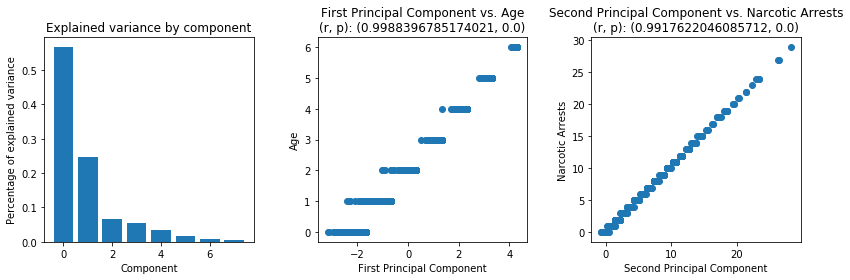
\includegraphics[scale=.55]{images/pca.png}}
In the public description of the CVRM, we find the remark that "inclusion of narcotics arrests and gang affiliation [has] only marginal impact on the results beyond what the model discerns from the other risk factors; therefore, in the current CVRM version, these two risk factors have been omitted."\cite{factsheet} If age and narcotic arrests capture most of the variance in the predictors as indicated by the figure above, the omission of narcotic arrests in the CVRM may reflect an understanding that narcotic arrests is approximately a weighted combination of other inputs.
\subsection{Predictor Strengths}
Recall \cite{upturn} found that age accounts for $89$\% of the variance in SSL score - unsurprisingly, age at latest arrest is by far the most important predictor across all our models. We can assess the relative importance of the predictors for our models concretely: a multiple linear regression on standardized predictors yields coefficients that are just the relative strengths of the predictors. Furthermore, we can assess a predictor's importance to a random forests regression by its total variance reduction across all nodes that split on that feature. Concretely, we have the below barplots.
\begin{center}
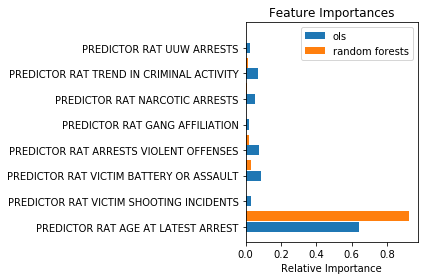
\includegraphics[scale=.7]{images/feature_importances.png}
\end{center}
In the linear model, age is the strongest predictor ($63.91$\% relative importance), while being a victim of a battery or assault is the second strongest predictor ($7.07$\%), followed by arrests for violent offenses ($6.04$\%) and trend in criminal activity ($5.75$\%). In a random forests regression, age is even more dominant at $92.67$\% relative importance - the next highest predictor, being a victim of a battery or assault, only has $2.80$\% relative importance.
\\\\
\newpage